\documentclass[12pt]{article}
\setlength{\oddsidemargin}{0in}
\setlength{\evensidemargin}{0in}
\setlength{\textwidth}{6.5in}
\setlength{\parindent}{0in}
\setlength{\parskip}{\baselineskip}

\usepackage{amsmath,amsfonts,amssymb,circuitikz,pdfpages}

\newcommand{\overbar}[1]{\mkern 1.5mu\overline{\mkern-1.5mu#1\mkern-1.5mu}\mkern 1.5mu}

\begin{document}
\title{Digital Logic Homework 2}

ECEN 2350 Spring 2017 \hfill Homework 2\\
Samuel Cuthbertson

\hrulefill

\begin{enumerate}

	\item \textit{Book Problems: 2.12, 2.13 and 2.14}
	\begin{enumerate}
    	
		\item[(2.12)] \textit{Find the minimum SOP expression for $f=x_1x_3 + x_1\overbar{x_2} + \overbar{x_1}x_2x_3 + \overbar{x_1}\overbar{x_2}\overbar{x_3}$}
    
    	\begin{align*}
        	f &= x_1x_3 + x_1\overbar{x_2} + \overbar{x_1}x_2x_3 + \overbar{x_1}\overbar{x_2}\overbar{x_3} \\
			f &= x_3(x_1+\overbar{x_1}x_2) + \overbar{x_2}(x_1 + \overbar{x_1}\overbar{x_3}) & \textit{Distributive} \\
            f &= x_3(x_1+x_2) + x_2(x_1+\overbar{x_3}) & \textit{DeMorgan's} \\
            f &= x_3x_1+x_3x_2+x_2x_1+x_2\overbar{x_3} & \textit{Distributive} \\
            \textit{For Consensus,}& \quad\textit{Note: $ab+bc+\overbar{a}c=ab+\overbar{a}c$}\\
            \textit{For Consensus,}& \quad\textit{Let: $a=x_3$, $b=x_1$, and $c=x_2$}\\
            \textit{For Consensus,}& \quad\textit{Substitute $x_3x_1+x_1x_2+x_2\overbar{x_3}$ for $x_3x_1+x_2\overbar{x_3}$}\\
            f &= x_3x_1+x_3x_2+x_2\overbar{x_3} & \textit{Consensus} \\
            f &= \boxed{\mathbf{x_3x_1+x_3x_2+x_2\overbar{x_3}}}
    	\end{align*}
    
    	\item[(2.13)] \textit{Find the minimum SOP expression for $f=x_1\overbar{x_2}\overbar{x_3} + x_1x_2x_4 + x_1\overbar{x_2}x_3\overbar{x_4}$}
    	\begin{align*}
    	f &= x_1\overbar{x_2}\overbar{x_3} + x_1x_2x_4 + x_1\overbar{x_2}x_3\overbar{x_4} \\
        f &= x_1(\overbar{x_2}\overbar{x_3} + x_2x_4 + \overbar{x_2}x_3\overbar{x_4}) & \textit{Distributive} \\
        f &= x_1(\overbar{x_2}(\overbar{x_3}+x_3\overbar{x_4}) + x_2x_4) & \textit{Distributive} \\
        f &= x_1(\overbar{x_2}(\overbar{x_3}+\overbar{x_4}) + x_2x_4) & \textit{DeMorgan's} \\
        f &= x_1(\overbar{x_2}\overbar{x_3}+\overbar{x_2}\overbar{x_4} + x_2x_4) & \textit{Distributive} \\
        f &= x_1\overbar{x_2}\overbar{x_3}+x_1\overbar{x_2}\overbar{x_4} + x_1x_2x_4 & \textit{Distributive} \\
        f &= \boxed{\mathbf{x_1\overbar{x_2}\overbar{x_3}+x_1\overbar{x_2}\overbar{x_4} + x_1x_2x_4}} \\
    	\end{align*}

		\newpage
    	\item[(2.14)] \textit{Find the minimum POS expression for $f=(x_1+x_3+x_4)(x_1+\overbar{x_2}+x_3)(x_1+\overbar{x_2}+\overbar{x_3}+x_4)$}
    	\begin{align*}
    	f &= (x_1+x_3+x_4)(x_1+\overbar{x_2}+x_3)(x_1+\overbar{x_2}+\overbar{x_3}+x_4) \\
    	\overbar{f} &= \overbar{(x_1+x_3+x_4)(x_1+\overbar{x_2}+x_3)(x_1+\overbar{x_2}+\overbar{x_3}+x_4)} \\
    	\overbar{f} &= \overbar{(x_1+x_3+x_4)}+\overbar{(x_1+\overbar{x_2}+x_3)}+\overbar{(x_1+\overbar{x_2}+\overbar{x_3}+x_4)} & \textit{DeMorgan's} \\
        \overbar{f} &= (\overbar{x_1}\overbar{x_3}\overbar{x_4})+(\overbar{x_1}\overbar{\overbar{x_2}}\overbar{x_3})+(\overbar{x_1}\overbar{\overbar{x_2}}\overbar{\overbar{x_3}}\overbar{x_4}) & \textit{DeMorgan's}\\
        \overbar{f} &= (\overbar{x_1}\overbar{x_3}\overbar{x_4})+(\overbar{x_1}x_2\overbar{x_3})+(\overbar{x_1}x_2x_3\overbar{x_4}) & \textit{Single Variable Thrm}\\
        \overbar{f} &= (\overbar{x_1}\overbar{x_3}\overbar{x_4})+(\overbar{x_1}x_2\overbar{x_3})+(\overbar{x_1}x_2x_3\overbar{x_4})+(\overbar{x_1}x_2x_3\overbar{x_4}) & \textit{Repeating Term}\\
        \overbar{f} &= \overbar{x_1}(\overbar{x_3}\overbar{x_4}+x_2\overbar{x_3}+x_2x_3\overbar{x_4}+x_2x_3\overbar{x_4}) & \textit{Distributive}\\
        \overbar{f} &= \overbar{x_1}(\overbar{x_4}(\overbar{x_3}+x_2x_3)+x_2(\overbar{x_3}+x_3\overbar{x_4})) & \textit{Distributive}\\
        \overbar{f} &= \overbar{x_1}(\overbar{x_4}(\overbar{x_3}+x_2)+x_2(\overbar{x_3}+\overbar{x_4})) & \textit{DeMorgan's}\\
        \overbar{f} &= \overbar{x_1}(\overbar{x_4}\overbar{x_3}+\overbar{x_4}x_2+x_2\overbar{x_3}+x_2\overbar{x_4}) & \textit{Distributive}\\
        \overbar{f} &= \overbar{x_1}(\overbar{x_4}\overbar{x_3}+\overbar{x_4}x_2+x_2\overbar{x_3}) & \textit{Distributive}\\
        \overbar{f} &= \overbar{x_1}\overbar{x_4}\overbar{x_3}+\overbar{x_1}\overbar{x_4}x_2+\overbar{x_1}x_2\overbar{x_3} & \textit{Distributive}\\
        \overbar{\overbar{f}} &= \overbar{\overbar{x_1}\overbar{x_4}\overbar{x_3}+\overbar{x_1}\overbar{x_4}x_2+\overbar{x_1}x_2\overbar{x_3}} \\
       	f &= (\overbar{\overbar{x_1}\overbar{x_4}\overbar{x_3}})(\overbar{\overbar{x_1}\overbar{x_4}x_2})(\overbar{\overbar{x_1}x_2\overbar{x_3}}) & \textit{DeMorgan's}\\
        f &= \boxed{\mathbf{(x_1+x_4+x_3)(x_1+x_4+\overbar{x_2})(x_1+\overbar{x_2}+x_3)}} & \textit{DeMorgan's}\\
    	\end{align*}
    
	\end{enumerate}
	
        
    \newpage
    \item \textit{Given the truth table below, answer the following:}
	\begin{center}
    \begin{tabular}{ccc|c|c|c}
    a & b & c & f & minterm & maxterm \\
    \hline
    0 & 0 & 0 & 0 & $\overbar{a}\overbar{b}\overbar{c}$ & a+b+c \\
    0 & 0 & 1 & 1 & $\overbar{a}\overbar{b}c$ & $a+b+\overbar{c}$ \\
    0 & 1 & 0 & 0 & $\overbar{a}b\overbar{c}$ & $a+\overbar{b}+c$\\
    0 & 1 & 1 & 1 & $\overbar{a}bc$ & $a+\overline{b}+\overline{c}$ \\
    1 & 0 & 0 & 1 & $a\overbar{b}\overbar{c}$ & $\overline{a}+b+c$ \\
    1 & 0 & 1 & 0 & $a\overbar{b}c$ & $\overline{a}+b+\overline{c}$\\
    1 & 1 & 0 & 1 & $ab\overbar{c}$ & $\overline{a}+\overline{c}+c$ \\
    1 & 1 & 1 & 1 & $abc$ & $\overbar{a}+\overbar{b}+\overbar{c}$\\
    \end{tabular}
	\end{center}    
    
    \begin{enumerate}
    	\item \textit{Provide the canonical sum of products logic equation for f(a,b,c)}

		The canonical sum of products logic equation for $f$ is given by taking the minterms from every line where $f(a,b,c)=1$, and combining them into this:
        \begin{align*}
        	f(a,b,c) &= \boxed{\mathbf{\overbar{a}\overbar{b}c + \overbar{a}bc + a\overbar{b}\overbar{c} + ab\overbar{c} + abc}}
        \end{align*}
        
    	\item \textit{Using Boolean algebra, derive the minimum cost sum-of-products logic equation for $f$. Specify which axiom, theorems, and properties were used for each step. Report the cost (number of gates and inputs).}
		\begin{align*}
        	f(a,b,c) &= \overbar{a}\overbar{b}c + \overbar{a}bc + a\overbar{b}\overbar{c} + ab\overbar{c} + abc \\
            f(a,b,c) &= \overbar{a}c(\overbar{b}+b) + a\overbar{c}(\overbar{b}+b) + abc & \textit{Distributive} \\
            f(a,b,c) &= \overbar{a}c(1) + a\overbar{c}(1) + abc & \textit{Single Variable Thrm} \\
            f(a,b,c) &= c(ba+\overbar{a}) + a\overbar{c} & \textit{Distributive} \\
            f(a,b,c) &= c(b+\overbar{a}) + a\overbar{c} & \textit{DeMorgan's} \\
            f(a,b,c) &= cb + c\overbar{a} + a\overbar{c} & \textit{Distributive} \\
            f(a,b,c) &= \boxed{\mathbf{cb + c\overbar{a} + a\overbar{c}}} \\
        \end{align*}
        As the answer has a, b and c feeding into three $and$ gates which feed into an $or$ gates, and only two of the outputs are inverted, the circuit has $3+2*1+3*2+1*3=14$ inputs and $3+1+2=6$ gates for a cost of $14+6=\boxed{\textbf{20}}$ \\
        
        \newpage
    	\item \textit{Synthesize (draw the gates) the minimum cost sum-of-products circuit for the logic equation obtained above.}
		\begin{center}
			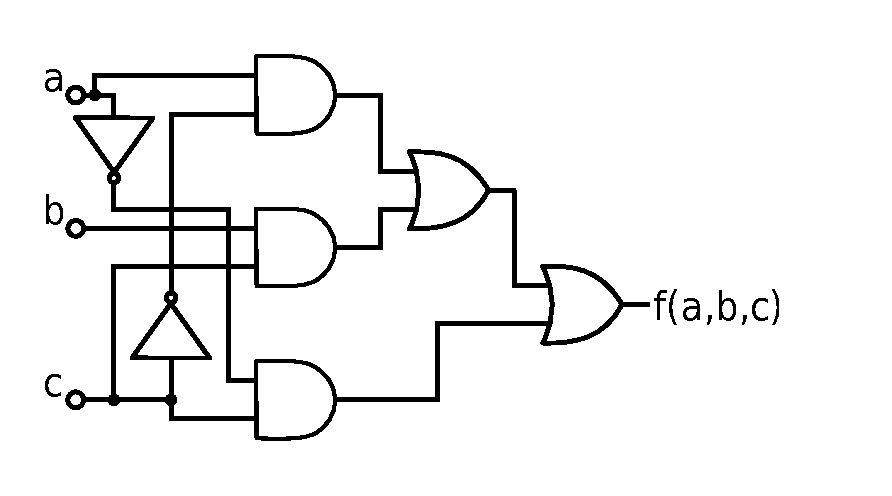
\includegraphics[scale=0.5]{circuit1.pdf}
		\end{center}
    	\end{enumerate} 
    
    \item \textit{Given the Truth Table above, answer the following:} 
    
	\begin{enumerate}
		\item \textit{Provide the canonical product of sums logic equation for f(a,b,c)} 
        
		The canonical product of sums logic equation for $f$ is given by taking the maxterms from every line where $f(a,b,c)=0$, and combining them into this:
        \begin{align*}
        	f(a,b,c) &= \boxed{\mathbf{(a+b+c)(a+\overbar{b}+c)(\overline{a}+b+\overline{c})}}
        \end{align*}
		
        
		\item \textit{Using Boolean algebra, derive the minimum cost product-of-sums logic equation for $f$. Specify which axiom, theorems, and properties were used for each
step. Report the cost (number of gates and inputs).}
		\begin{align*}
        	f(a,b,c) &= (a+b+c)(a+\overbar{b}+c)(\overline{a}+b+\overline{c}) \\
        	f(a,b,c) &= (a+c)(a+c)(\overline{a}+b+\overline{c}) & \textit{Combining} \\
        	f(a,b,c) &= (a+c)(\overline{a}+b+\overline{c}) & \textit{Simplification} \\
            f(a,b,c) &= \boxed{\mathbf{(a+c)(\overline{a}+b+\overline{c})}}
        \end{align*}
        As the answer has a, b and c feeding into two $or$ gates which feed into one $and$ gate and two of the inputs are inverted, the circuit has $3+2*1+2*2+3*1=12$ inputs and $2+2+2=6$ gates for a total cost of $12+6=\boxed{\mathbf{18}}$ \\

		\newpage
		\item \textit{Synthesize (draw the gates) the minimum cost product-of-sums circuit for the logic
equation obtained above.}
		\begin{center}
			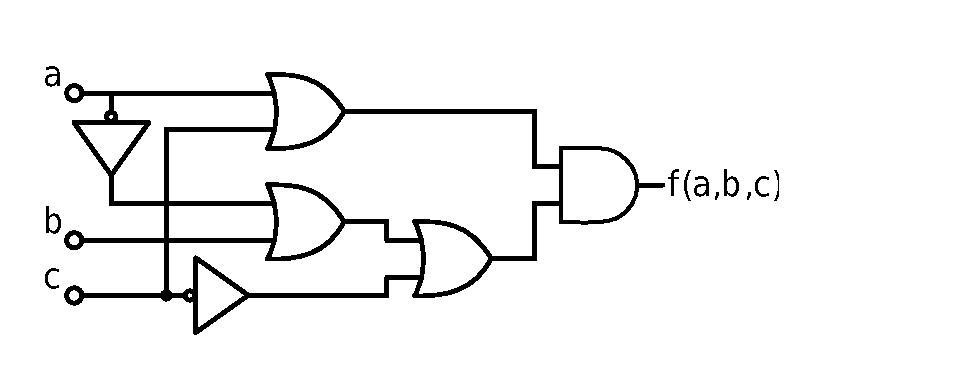
\includegraphics[scale=0.5]{circuit2.pdf}
		\end{center}
        
	\end{enumerate}

		
\end{enumerate}


\end{document}

